%% Elsevier CAS single-column template
%% Manuscript: Adjoint transport theory for rare-event sampling in spin systems
%% Shortened revision: [E]/[V]/[O] claim grading removed, open-question sections
%% removed, paragraphs consolidated.

\documentclass[a4paper,fleqn]{cas-sc}

%% ---- Citation / bibliography style -------------------------------------
\usepackage[numbers,sort&compress]{natbib}
\usepackage{rotating}
\usepackage{booktabs}
\usepackage{amsmath}
\usepackage{graphicx}
\usepackage{caption}   % enables \captionof for non-floating figures
\usepackage{float}     % enables [H] placement option
\usepackage{placeins}  % \FloatBarrier confines floats to their section

%% ---- Packages carried over from the original manuscript ----------------
\usepackage{amssymb}
\usepackage{enumitem}
\usepackage{xcolor}
\usepackage{tikz}
\usetikzlibrary{arrows.meta,positioning,calc}
\definecolor{acc}{HTML}{2c5aa0}
\setlist{itemsep=2pt,topsep=3pt}
\newtheorem{claim}{Claim}
\newtheorem{prop}{Proposition}
\newcommand{\dg}{^{\dagger}}
\newcommand{\ip}[2]{\langle #1,\,#2\rangle}
\newcommand{\E}{\mathbb{E}}

\begin{document}
	\let\WriteBookmarks\relax
	\def\floatpagepagefraction{1}
	\def\textpagefraction{.001}
	
	% Short title (running head)
	\shorttitle{Adjoint-importance rare-event sampling in spin systems}
	
	% Short author
	\shortauthors{M.Y. Alzaatreh}
	
	% Main title
	\title[mode=title]{From Radiation Shielding to Spin Glasses: Auditing the Adjoint-Importance Toolkit for Rare-Event Sampling}
	
	% ---- Authors -----------------------------------------------------------
	\author{M.Y. Alzaatreh}
	
	\affiliation{organization={Natural Sciences Unit, Fahad Bin Sultan University},
		city={Tabuk},
		country={Saudi Arabia}}
	
	% ---- Abstract ----------------------------------------------------------
	\begin{abstract}
		This work transfers the adjoint-importance toolkit of radiation shielding to spin systems, testing it end to end on the 2D Ising ferromagnet and the Edwards--Anderson spin glass. The identity between the transport adjoint and the rare-event committor is exact and is verified to machine precision. Weighted Ensemble, the statistical-mechanics analogue of split/roulette weight windows, is validated against exact enumeration and reaches two decades deeper into the tail than naive Monte Carlo at matched cost. A learned importance coordinate proves sensitive to network initialization: across seventeen independent retrainings, a two-level bootstrap gives a geometric-mean figure-of-merit ratio of $1.19\times$ (95\% CI $[0.84,1.75]$) against the best hand-picked coordinate, a positive but not significant effect. A deep-ensemble follow-up, which attacks the diagnosed noise source (weight initialization) directly rather than adding more single-net seeds, reduces the run-to-run spread as intended but converges toward a loss; correcting a cost-accounting gap the ensemble exposes --- neural-network inference cost had been silently uncounted --- makes that loss statistically decisive ($0.087\times$, 95\% CI $[0.051,0.155]$), the only comparison in this paper whose confidence interval excludes parity. A label-free self-consistency objective from recent neural importance-function work likewise yields a favourable point estimate that does not survive bootstrap replication. FW-CADIS global allocation matches the error profile of uniform allocation at roughly one-eighth the simulation cost, although the flattening of relative error for which it is named is not observed at the scales tested. Naive Monte Carlo remains the most efficient estimator up to $L=32$, placing the tested rarity regime below the crossover at which variance-reduction overhead is repaid. Together these results establish a validated transfer of the transport sampling machinery to spin systems, delimit its present practical limits, and supply a reproducible benchmark and statistical discipline for future work.
	\end{abstract}
	
	% ---- Highlights ---------------------------------------------------------
	\begin{highlights}
		\item Transport adjoint importance and the rare-event committor are identical; verified to machine precision.
		\item Weighted Ensemble validated against exact enumeration; two decades deeper than naive Monte Carlo.
		\item FW-CADIS attains equivalent threshold coverage at roughly one-eighth the allocation cost.
		\item Learned importance coordinate gives a $1.19\times$ FOM ratio, bounded by a two-level bootstrap.
		\item Deep ensembling resolves that ambiguity as a decisive $0.087\times$ loss (95\% CI $[0.051,0.155]$).
		\item Naive Monte Carlo wins at every lattice size up to $L=32$, with no narrowing margin.
	\end{highlights}
	
	% ---- Keywords ----------------------------------------------------------
	\begin{keywords}
		Rare-event sampling \sep Adjoint transport \sep Committor function \sep Weighted Ensemble \sep FW-CADIS \sep Variance reduction \sep Spin systems
	\end{keywords}
	
	\maketitle
	
	% ========================================================================
	\section{Introduction}\label{sec:intro}
	Rare-event sampling is the shared computational difficulty of two literatures that rarely
	cite one another. Weighted Ensemble, Forward Flux Sampling and committor-based methods are
	already the working tools for nucleation, protein folding and reaction-rate calculation
	\cite{allen2009, zuckerman2017, e2006}, and the obstacle they all face is structural: an
	unbiased estimator of an event of probability $p$ has relative error of order $(Np)^{-1/2}$,
	so each decade of rarity costs an order of magnitude in computing
	\cite{allen2009, touchette2009}. Every serious remedy therefore replaces more samples with
	better-placed ones, an idea present in Monte Carlo since importance sampling and trajectory
	splitting \cite{kahn1951, kahn1953}.
	
	Radiation transport met the problem first, in deep-penetration shielding, where analog
	scoring probabilities fall below $10^{-10}$ \cite{spanier1969, wagner1998}. Its remedy is the
	\emph{adjoint} flux, or importance function, which runs the transport equation backwards from
	the detector response to give the expected contribution of a particle at each phase-space
	point \cite{lewins1965, bell1970}, and is then used both to bias source emission and to set
	weight windows, inside which particles are split and outside which they are killed by Russian
	roulette \cite{kahn1951, booth1984}. CADIS automated this by deriving both devices
	consistently from a coarse deterministic adjoint, giving figure-of-merit gains of several
	orders of magnitude on realistic geometries \cite{wagner1998, haghighat2003}; its
	forward-weighted extension FW-CADIS replaces the single-detector objective with a
	\emph{global} one, seeking uniform uncertainty across a whole family of responses
	\cite{wagnerfw2014, cooper2001}. Performance is judged throughout by the figure of merit
	$\mathrm{FOM}=1/(\sigma_{\mathrm{rel}}^{2}T)$, a cost-normalised inverse variance
	\cite{spanier1969, wagnerfw2014}.
	
	Statistical mechanics reached closely related tools independently. Transition Path Theory
	describes reactive trajectories through the committor $h(s)$, the probability of reaching a
	target set before returning to the origin set, which is the optimal reaction coordinate in a
	precise sense \cite{e2006, metzner2009, evanden2010}; its practical samplers are splitting
	methods in disguise, whether by splitting and merging weighted replicas across bins
	\cite{huber1996, zhang2010}, advancing an ensemble through fixed or adaptive interfaces
	\cite{allen2009, cerou2007}, or working directly in trajectory space \cite{bolhuis2002}. What
	unites and limits them is dependence on a user-supplied coordinate, with no general
	prescription for choosing it \cite{zuckerman2017, allen2009}. Lattice spins are the natural
	testbed for that limitation: the 2D Ising ferromagnet \cite{ising1925} has an exact solution
	to validate against \cite{onsager1944}, while the Edwards--Anderson model adds quenched
	disorder, frustration and no obvious coordinate \cite{edwards1975, binder1986}. Both are
	usually simulated with Metropolis dynamics \cite{metropolis1953}, whose critical slowing down
	motivated cluster updates \cite{swendsen1987, wolff1989} and flat-histogram schemes
	\cite{berg1992, wanglandau2001} --- methods that flatten a free-energy landscape rather than
	steer trajectories toward a specified tally, and so optimise a mismatched objective here
	\cite{wanglandau2001}.
	
	That the two importance functions coincide is classical rather than new: both are instances
	of Doob's $h$-transform \cite{doob1984}, which reappears as the driven process of
	large-deviation theory underpinning the zero-variance sampler
	\cite{chetrite2015, touchette2009} and, in stochastic-control form, as the solution of a
	Gibbs variational principle \cite{hartmann2019}. Machine learning has supplied a third route.
	Physics-informed networks solve high-dimensional PDEs without a grid \cite{raissi2019}, and
	were applied to the committor equation itself \cite{li2019, khoo2019}, with active importance
	sampling concentrating training effort where rarely visited regions dominate the loss
	\cite{rotskoff2020}; a separate line trains a committor variationally and uses it as a
	metadynamics-like collective variable with a bias potential rather than a weight-window
	schedule \cite{trizio2025}. Generative models were meanwhile trained directly on spin systems
	--- variational autoregressive networks \cite{wu2019} and Boltzmann generators
	\cite{noe2019} --- with later work recovering unbiased observables by reweighting
	\cite{nicoli2020} or embedding the model in a Markov chain \cite{gabrie2022}.
	
	The gap this leaves is specific. The identity is established \cite{doob1984, chetrite2015} and
	neural committors exist \cite{li2019, khoo2019, trizio2025}, but the transport \emph{toolkit}
	built around that identity --- consistent weight windows, the global FW-CADIS objective, the
	FOM as an evaluation standard --- was designed for precisely the regime where
	learned-committor methods are weakest \cite{wagner1998, wagnerfw2014}, and has never been
	transferred to spin systems and audited. Every neural-committor line above samples by
	continuously reweighting or biasing dynamics rather than by the transport toolkit's discrete
	population control: splitting a walker, killing it by roulette, resampling to a fixed per-bin
	occupancy. The closest prior work makes the point concretely. Kim and Cai \cite{kim2026}
	learn an importance function $I(s)$, modify transitions as $K'(i\to j)=K(i\to j)I(j)/I(i)$,
	and use a branching random walk --- in the language of \S\ref{sec:identity}, their $I$ is our
	$h$, their $K'$ is the tilt, and their branching is splitting, so they independently
	reconstruct the zero-variance/weight-window recipe for discrete rare transitions without the
	transport framing, and without comparing their learned coordinate against a hand-picked one.
	Their self-consistency objective is implemented and tested directly here
	(\S\ref{sec:kimcai}).
	
	This paper builds and audits the transport toolkit end to end on the 2D Ising ferromagnet,
	where a good reaction coordinate is known in advance, and the Edwards--Anderson spin glass,
	where the obvious candidate carries almost no information, treating each piece of machinery as
	a hypothesis rather than a technique to be demonstrated. The adjoint$=$committor identity
	holds to numerical precision; the empirical claims built on it --- that weight windows reach
	usefully deeper into the tail, that a learned importance coordinate beats a hand-picked one,
	that FW-CADIS flattens relative error across a family of thresholds, and that any of this
	earns back its overhead at reachable lattice sizes --- fared less uniformly, and are reported
	as found, with a bootstrap confidence interval attached to every comparative claim.
	
	\FloatBarrier
	
	% ========================================================================
	\section{Materials and Methods}\label{sec:methods}
	
	Figure~\ref{fig:pipeline} summarises the pipeline end to end; the rest of this section
	describes each stage in turn.
	
	% --- FIGURE 1 ---
	\noindent
	\begin{minipage}{\linewidth}
		\centering
		\hyphenpenalty=10000 \exhyphenpenalty=10000
		\thinmuskip=3mu \medmuskip=4mu \thickmuskip=5mu
		\resizebox{\linewidth}{!}{%
			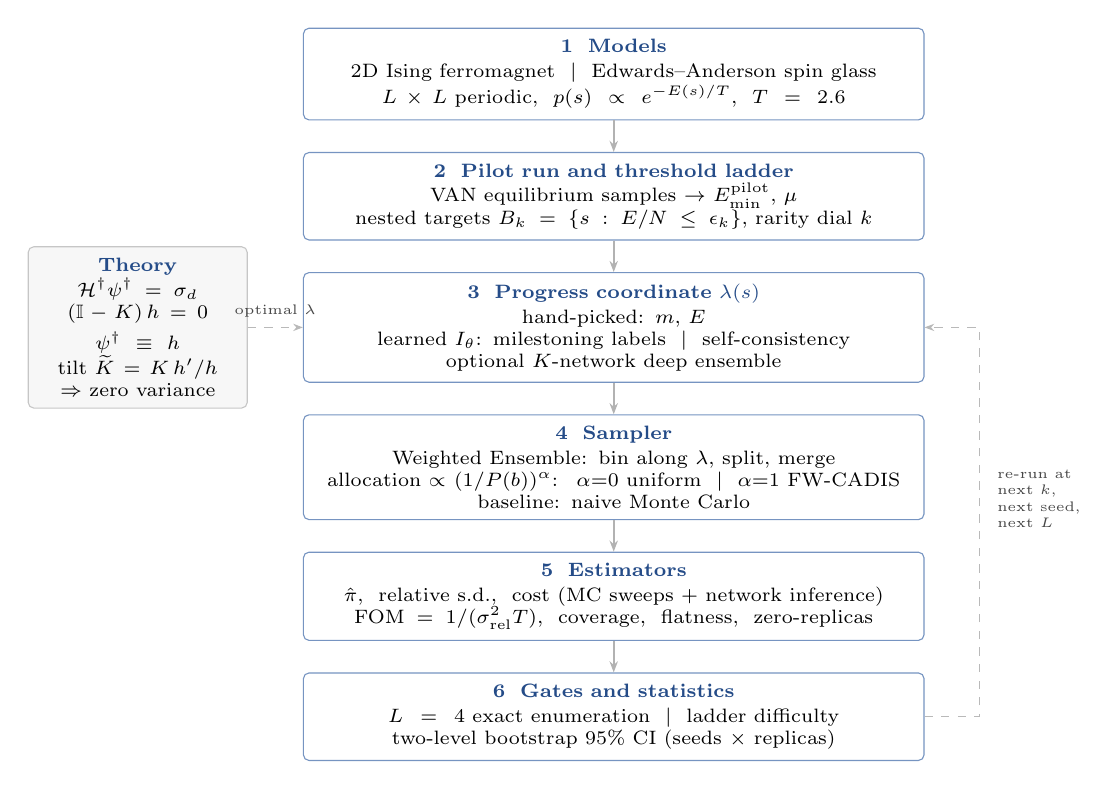
\begin{tikzpicture}[
				font=\scriptsize,
				stage/.style={draw=acc!65,rounded corners=2pt,align=center,inner sep=4pt,
					text width=76mm,fill=white},
				side/.style={draw=gray!45,rounded corners=2pt,align=center,inner sep=4pt,
					text width=25mm,fill=gray!6},
				flow/.style={-{Stealth[length=4pt]},thick,gray!60},
				aux/.style={-{Stealth[length=3.5pt]},gray!55,dashed},
				node distance=4mm,
				]
				\node[stage] (models) {\textcolor{acc!85!black}{\textbf{1\ \ Models}}\\[1pt]
					2D Ising ferromagnet \ $|$ \ Edwards--Anderson spin glass\\
					$L\times L$ periodic, \ $p(s)\propto e^{-E(s)/T}$, \ $T=2.6$};
				
				\node[stage,below=of models] (pilot) {\textcolor{acc!85!black}{\textbf{2\ \ Pilot run and threshold ladder}}\\[1pt]
					VAN equilibrium samples $\rightarrow$ $E^{\rm pilot}_{\min}$, $\mu$\\
					nested targets $B_k=\{s:E/N\le\epsilon_k\}$, rarity dial $k$};
				
				\node[stage,below=of pilot] (coord) {\textcolor{acc!85!black}{\textbf{3\ \ Progress coordinate $\lambda(s)$}}\\[1pt]
					hand-picked: $m$, $E$\\
					learned $I_\theta$: milestoning labels \ $|$ \ self-consistency\\
					optional $K$-network deep ensemble};
				
				\node[stage,below=of coord] (sampler) {\textcolor{acc!85!black}{\textbf{4\ \ Sampler}}\\[1pt]
					Weighted Ensemble: bin along $\lambda$, split, merge\\
					allocation $\propto(1/P(b))^{\alpha}$: \ $\alpha{=}0$ uniform \ $|$ \ $\alpha{=}1$ FW-CADIS\\
					baseline: naive Monte Carlo};
				
				\node[stage,below=of sampler] (est) {\textcolor{acc!85!black}{\textbf{5\ \ Estimators}}\\[1pt]
					$\hat\pi$, \ relative s.d., \ cost (MC sweeps $+$ network inference)\\
					$\mathrm{FOM}=1/(\sigma_{\rm rel}^{2}T)$, \ coverage, \ flatness, \ zero-replicas};
				
				\node[stage,below=of est] (gates) {\textcolor{acc!85!black}{\textbf{6\ \ Gates and statistics}}\\[1pt]
					$L=4$ exact enumeration \ $|$ \ ladder difficulty\\
					two-level bootstrap 95\% CI (seeds $\times$ replicas)};
				
				\foreach \a/\b in {models/pilot,pilot/coord,coord/sampler,sampler/est,est/gates}
				{\draw[flow] (\a) -- (\b);}
				
				\node[side,left=7mm of coord] (theory) {\textcolor{acc!85!black}{\textbf{Theory}}\\[1pt]
					$\mathcal H\dg\psi\dg=\sigma_d$\\ $(\mathbb I-K)\,h=0$\\[2pt]
					$\psi\dg\equiv h$\\ tilt $\widetilde K=K\,h'/h$\\ $\Rightarrow$ zero variance};
				\draw[aux] (theory.east) -- node[above,font=\tiny,gray!55!black]{optimal $\lambda$} (coord.west);
				
				\coordinate (r) at ($(gates.east)+(7mm,0)$);
				\draw[aux] (gates.east) -- (r) |- node[right,font=\tiny,gray!55!black,pos=0.28,
				align=left,xshift=1mm]{re-run at\\next $k$,\\next seed,\\next $L$} (coord.east);
		\end{tikzpicture}}
		\captionof{figure}{The system end to end. A pilot run fixes a nested ladder of rare-energy
			targets; a progress coordinate --- hand-picked or learned --- is chosen; Weighted
			Ensemble bins walkers along it and splits or merges them under one of two allocation
			rules; and the resulting estimator is scored on figure of merit, coverage and flatness.
			Every comparison passes the gates of stage 6 before it is reported. The theory panel
			(left) is what licenses the whole construction: the transport adjoint and the committor
			solve the same equation, so tilting by it is zero-variance, and stage 3 is an attempt to
			approximate that ideal coordinate. The dashed return path is the outer loop over target
			depth $k$, network seed and lattice size $L$.}
		\label{fig:pipeline}
	\end{minipage}
	\par\vspace{0.8\baselineskip}
	
	\subsection{Theory: the adjoint$=$committor identity}\label{sec:theory}
	
	\subsubsection{Linear transport and the adjoint importance function}
	Let $P=(\mathbf r,\mathbf\Omega,E)$ be a phase-space point and $\psi(P)$ the particle flux
	obeying the linear transport (Boltzmann) equation, written abstractly as $\mathcal H\,\psi
	= q$, with transport operator $\mathcal H$ (streaming $+$ collision) and source $q$. A
	detector response (``tally'') is a linear functional $R=\ip{\sigma_d}{\psi}=\int
	\sigma_d(P)\,\psi(P)\,dP$, where $\sigma_d$ is the detector cross-section. Define the
	\emph{adjoint} flux $\psi\dg$ by
	\begin{equation}
		\mathcal H\dg\,\psi\dg=\sigma_d .
		\label{eq:adjoint}
	\end{equation}
	The defining property of the adjoint gives the fundamental identity
	\begin{equation}
		\boxed{\;R=\ip{\sigma_d}{\psi}=\ip{\psi\dg}{q}\;}
		\label{eq:fund}
	\end{equation}
	and the physical reading that makes everything work: $\psi\dg(P)$ is the expected
	contribution to the tally $R$ of a single particle introduced at $P$ --- its
	\emph{importance}. If one samples particle transitions biased toward high importance and
	assigns each particle the statistical weight $w(P)\propto 1/\psi\dg(P)$, then, when
	$\psi\dg$ is exact, every history contributes an identical score and the estimator of $R$
	has \emph{zero variance}. This is the theoretical ceiling of variance reduction; all
	practical schemes approximate it.
	
	\subsubsection{CADIS, FW-CADIS, weight windows, figure of merit}
	Since $\psi\dg$ is unknown, CADIS (Consistent Adjoint-Driven Importance Sampling) computes
	a cheap, approximate $\psi\dg$ and uses it to drive an expensive forward Monte Carlo run
	through two consistent devices: \textbf{source biasing}, sampling from
	$\hat q(P)=\psi\dg(P)q(P)/R$ instead of $q$; and \textbf{weight windows}, assigning each
	phase-space cell a target weight $w\propto 1/\psi\dg$ and a window
	$[w_{\text{target}}/k,\,k\,w_{\text{target}}]$ --- a particle above the window is
	\emph{split} into equal-weight copies, one below is \emph{Russian-rouletted}. This keeps
	$w(P)\,\psi\dg(P)\approx\text{const}$, bounding the weight and hence the variance.
	\textbf{FW-CADIS} (forward-weighted CADIS) extends this to \emph{global} variance
	reduction: weighting the adjoint source by the inverse of the local forward response
	produces weight windows that equalise \emph{relative} statistical error across many
	detectors, or the whole domain, at once, rather than optimising a single tally. Efficiency
	is measured by the figure of merit $\mathrm{FOM}=1/(\sigma_{\mathrm{rel}}^2\,T)$, the
	inverse product of relative variance and CPU time.
	
	\subsubsection{The central identity: importance $=$ committor $=$ zero-variance measure}\label{sec:identity}
	Work with a Markov chain on configurations $s$ with transition kernel $K(s\to s')$. Let $A$
	(failure/bulk) and $B$ (the rare target set) be disjoint, and define the \textbf{committor}
	$h(s)=\Pr[\text{reach }B\text{ before }A\mid\text{start at }s]$, with $h|_A=0$, $h|_B=1$.
	On the transient set it satisfies the discrete backward equation
	\begin{equation}
		h(s)=\sum_{s'}K(s\to s')\,h(s')\qquad\Longleftrightarrow\qquad (\mathbb I-K)\,h=0 .
		\label{eq:committor}
	\end{equation}
	Equation~\eqref{eq:committor} is precisely the discrete adjoint transport
	equation~\eqref{eq:adjoint} with the target set playing the role of the detector. Hence the
	rare-event committor $h(s)$, the transport adjoint importance $\psi\dg(s)$ (with
	$\sigma_d=\mathbf 1_B$), and the ``neural importance function'' of recent ML papers are the
	same function: the expected contribution of a walker at $s$ to the rare tally. Defining the
	tilted kernel $\widetilde K(s\to s')=K(s\to s')\,h(s')/h(s)$, the path likelihood ratio
	telescopes to $W=h(s_0)/h(s_{\text{end}})=h(s_0)$ for every path ending in $B$: every sample
	returns the identical value $h(s_0)=\pi$, so the estimator of $\pi$ has zero variance.
	
	Of the two readings of $\pi$ available here, this paper always means the second. The
	\emph{static} equilibrium mass $\Pr_{\rm eq}(s\in B)=\sum_{s\in B}p(s)$ is a property of the
	stationary measure alone, answerable by direct enumeration with no dynamics at all --- our
	$L=4$ gate (\S\ref{sec:validation}) computes exactly this. The \emph{dynamical} hitting
	probability $h(s_0)$ from a fixed bulk reference state $s_0\in A$ is what every $\hat\pi$
	reported in \S\ref{sec:results} estimates, and what Weighted Ensemble is built to sample
	efficiently. The two coincide under the same mixing condition transition-path theory
	already requires \cite{e2006}: dynamics equilibrates within $A$ faster than it escapes
	toward $B$, which holds throughout the $T=2.6>T_c$ regime tested here, though not
	necessarily at low temperature where $A$ could itself fragment into sub-basins.
	
	The construction was checked numerically on a solvable 1D walk before any spin-system code
	was written (\S\ref{sec:validation}); the outcome of that check is why every
	learned-coordinate result below uses Weighted Ensemble rather than pure importance
	reweighting.
	
	\subsubsection{Scope and limits of the correspondence}\label{sec:scope}
	The identity above is exact at the level of linear algebra, not merely structurally
	similar. Production transport codes do not solve the continuous operator
	equation~\eqref{eq:adjoint} directly: phase space is first discretized into energy groups
	and a finite set of directions \cite{wagner1998, lewins1965}, reducing it to a finite
	linear system $(\mathbb I-\mathbf K)\boldsymbol\psi\dg=\boldsymbol\sigma_d$ for a
	transition operator $\mathbf K$ packaging streaming and scattering between cells --- term
	for term the same system as Eq.~\eqref{eq:committor}. Nothing about $K$'s physical origin
	enters that algebra, which is why the identity transfers to spin dynamics with no
	modification to the mathematics: it holds for \emph{any} Markov process with an absorbing
	target set. What does not transfer is the physical mechanism generating $K$. Transport's
	$K$ encodes free flight interrupted by scattering and absorption at rates set by
	cross-sections; spin dynamics' $K$ encodes single-spin-flip acceptance under a thermal bath
	at temperature $T$. There is no mean free path or cross-section in the spin problem, and a
	``walker'' is a bookkeeping device for one member of a population of independent simulation
	replicas, not a physical particle.
	
	Two asymmetries follow, in opposite directions. Spin systems are the \emph{easier} problem
	in one specific sense: multigroup/discrete-ordinates transport carries a discretization
	error that must be checked against measurement, since the exact continuous answer is rarely
	available at all, whereas a spin lattice's state space is already finite ($2^N$
	configurations, no truncation) --- which is why $L=4$ can be checked against exact
	enumeration directly (\S\ref{sec:validation}). They are \emph{harder} in the place that matters
	most: transport bins its importance function along a natural, low-dimensional,
	physically meaningful coordinate --- position, direction, energy, fixed by the geometry of
	the shield --- while spin configurations have no such coordinate, and the obvious candidate,
	magnetization, fails outright on the spin glass (\S\ref{sec:models}). That absence, not the
	linear algebra, is why this paper needs a \emph{learned} importance coordinate
	(\S\ref{sec:objectives}) at all.
	
	\FloatBarrier
	
	\subsection{Models and threshold ladder}\label{sec:models}
	Two spin systems are used, both on an $L\times L$ square lattice with periodic boundaries
	and Gibbs measure $p(s)\propto e^{-E(s)/T}$: the \textbf{ferromagnet}
	($E=-J\sum_{\langle ij\rangle}s_is_j$, $J>0$), where the magnetization $m$ is an obviously
	informative reaction coordinate; and the \textbf{Edwards--Anderson (EA) spin glass}
	($J_{ij}=\pm J$ quenched-random per bond), whose low-energy states are disordered and
	frustrated so that $m\approx 0$ regardless of energy --- the case a hand-picked coordinate
	is expected to fail on, and the one this paper focuses its harder tests on. All results use
	$T=2.6$ (above $T_c\approx2.269$) unless noted; $L=16$ for full-scale results, $L=4$ for
	exact-enumeration gates. The \textbf{resampling interval $\tau$} (sweeps between WE
	split/merge operations) is stated explicitly throughout because it must be comparable to
	the system's own correlation time, $\tau_{\rm corr}\approx1$ sweep at $T=2.6$; otherwise
	splitting is undone by relaxation before the next resampling and every $\mathrm{WE}[\cdot]$
	variant degenerates silently toward naive Monte Carlo. Results using the \texttt{full}
	preset (\S\ref{sec:res-learned}, \S\ref{sec:kimcai}, \S\ref{sec:fwcadis}) use $\tau=4$;
	milestoning results (\S\ref{sec:milestone}) use $\tau=2$.
	
	\textbf{Threshold ladder.} Every rare-event target below is drawn from one nested family
	rather than chosen ad hoc per experiment. Given a pilot run's population, let
	$E^{\rm pilot}_{\min}$ be its deepest observed energy per spin and $\mu$ its bulk mean; the
	depth-$k$ target set is
	\begin{equation}
		B_k=\{s: E(s)/N\le\epsilon_k\},\qquad
		\epsilon_k=E^{\rm pilot}_{\min}-k\Delta,\qquad
		\Delta=\frac{\mu-E^{\rm pilot}_{\min}}{10},
		\label{eq:beyond}
	\end{equation}
	i.e.\ $k$ steps beyond the pilot's own most extreme observation, in units of one tenth of
	its observed dynamic range. This makes $k$ (\texttt{--beyond} throughout) a rarity dial
	portable across $L$, $T$, and disorder draw, and makes $B_k$ nested,
	$B_1\supset B_2\supset\cdots$ --- the structure both the FW-CADIS threshold family
	(\S\ref{sec:fwcadis}) and milestoning's progress labels (\S\ref{sec:milestone}) build on.
	The dial is genuine in practice, not just in principle: at fixed $L=16$, $T=2.6$, $\hat\pi$
	drops roughly one order of magnitude per step of $k$, and too large a $k$ places $B_k$
	outside what any method can resolve at the compute available, degrading every comparison to
	noise versus noise.
	
	\subsection{Samplers: variational autoregressive network and Weighted Ensemble}\label{sec:samplers}
	\textbf{Variational autoregressive network (VAN).} A normalized autoregressive neural network
	over spin configurations is trained variationally against the Gibbs measure, so that it draws
	statistically independent samples by construction rather than by decorrelating a Markov chain.
	Its role in this project is to remove critical slowing down near $T_c$, not to sample rare
	events; the two are different difficulties, and the VAN is used only as an equilibrium
	sampler.
	
	\textbf{Weighted Ensemble (WE).} WE is the statistical-mechanics name for split/Russian-roulette weight
	windows: a population of walkers, each carrying a weight, is periodically binned along a
	chosen coordinate; bins are equalised to a target occupancy by splitting
	over-weight bins and merging under-weight ones, conserving total weight exactly (hence unbiased for
	\emph{any} binning coordinate, good or bad). We validate the implementation against exact
	enumeration at $L=4$ before trusting any figure-of-merit comparison at scale.
	
	\subsection{Learned importance coordinates: two training objectives}\label{sec:objectives}
	A network $I_\theta(s)$ is trained to approximate the committor and then used as the WE
	binning coordinate, in place of a hand-picked one. Two training objectives are compared.
	
	\textbf{Surrogate rollout label (this project's default).} Binary committor labels collapse
	to all-zero for a genuinely rare target, so the network is instead trained to regress the
	\emph{best progress value reached} in $K$ short rollouts from each collected configuration
	--- a dense, monotone surrogate for the committor, not the committor itself. In its
	\textbf{milestoning} refinement, intermediate thresholds are placed along the ladder from
	bulk to target and a configuration's label estimates its committor to the \emph{next}
	milestone rather than to the final target directly, which stays closer to the theoretical
	object of \S\ref{sec:identity} while still avoiding all-zero label collapse.
	
	\textbf{Self-consistency (Kim \& Cai, 2026).} A label-free alternative: train $I_\theta$ by
	minimizing violation of its own self-consistency condition under the elementary
	single-spin-flip kernel, $\sum_j K(s\to j)\,I(j)=I(s)$, with boundary condition $I=1$ on the
	target. This equation, plus the target boundary alone, is under-determined: the constant
	solution $I\equiv1$ satisfies it everywhere, for any amount of training data. A second
	boundary condition --- anchoring bulk-equilibrium states to a distinct reference value ---
	breaks this degeneracy and is necessary, not optional.
	
	\subsection{FW-CADIS global allocation}
	Given a family of $K$ nested thresholds and a cheap pilot estimate of the equilibrium bin
	occupancy $P(b)$, FW-CADIS allocates walkers per bin $\propto (1/P(b))^\alpha$; $\alpha=0$
	recovers uniform allocation (the standard WE baseline), $\alpha=1$ is full FW-CADIS. Both
	settings use identical code, differing only in the allocation vector, which is what makes
	the comparison fair by construction. The metric is \textbf{coverage} first (how many of the
	$K$ thresholds were observed at all --- a method that fails a deep threshold has infinite
	error there, and scoring only the thresholds it survived would reward failure by making it
	look artificially flat) and \textbf{flatness} second, the spread (max/min) of relative error
	across the observed thresholds.
	
	\subsection{Statistical methodology}
	Two disciplines are applied uniformly and are largely responsible for this paper's
	qualified conclusions rather than overclaimed ones. \textbf{Ladder difficulty}: comparing
	methods in a regime where the baseline itself fails to observe the rare event (many
	zero-replicas) compares noise to noise, so every comparison below is reported at a depth
	where the reference method(s) reach 0, or close to 0, zero-replicas out of the replica
	count, found by backing off from a harder target until this holds.
	\textbf{Bootstrap confidence intervals}: a point-estimate ratio of figures of merit from a
	handful of replicas is not by itself evidence of a real effect, since FOM is a ratio
	involving a \emph{sample variance} that is itself noisy at small replica counts. Every
	comparative claim in \S\ref{sec:results} is therefore backed by a bootstrap 95\% confidence
	interval, resampling the replica axis with replacement, and claims that do not survive this
	check are reported as unresolved rather than smoothed into a verdict.
	
	\FloatBarrier
	
	% ========================================================================
	\section{Results and Discussion}\label{sec:results}
	
	\subsection{Validation against exact references}\label{sec:validation}
	Nothing below is compared on figure of merit until the machinery producing it has been
	checked against a reference whose answer is known independently.
	
	\textbf{The committor identity.} The committor identity of \S\ref{sec:identity} was checked on a solvable 1D absorbing
	random walk on $\{0,\dots,15\}$ before any lattice code was written, with the rare event
	(reaching state 15 before 0) calibrated to $\pi=1.14\times10^{-3}$. Tilting by the exact
	committor, available there in closed form, gave a measured relative variance of
	$\sim\!10^{-30}$ --- zero to machine precision, as the theory requires. Tilting by an
	\emph{approximate} committor under pure biasing, with no weight windows, was instead worse
	than naive Monte Carlo. That second outcome is why every subsequent learned-coordinate result
	in this paper uses Weighted Ensemble (split/roulette) rather than raw importance reweighting:
	an imperfect importance estimate, used to reweight without bounding the weights, can be
	actively harmful. It is also why deep-penetration transport uses weight windows rather than
	relying on reweighting alone.
	
	\textbf{Weighted Ensemble.} At $L=4$, WE reproduces the exact enumerated $P(m)$ to a mean $|\Delta\ln P|$ of
	0.006--0.024 across three tested regimes. At $L=20$, WE reaches roughly two decades deeper
	into the magnetization tail than naive Monte Carlo at matched cost: naive's hard floor is
	$|m|=0.886$ ($P\approx6\times10^{-6}$), where it returns zero samples and hence zero
	information; WE reaches $|m|=0.932$ ($P\approx2.4\times10^{-7}$). Separately, applying
	weight windows to that same approximate, otherwise-fragile tilt recovered roughly a $2\times$ figure-of-merit improvement
	over the same tilt without them (measured FOM $1.24\times10^{-5}\to4.86\times10^{-4}$) ---
	the robustness layer converts an actively harmful bias into a net improvement, exactly as
	the transport literature predicts. Magnetization is confirmed useless as a WE coordinate
	for the EA spin glass specifically: an early test recorded 10/10 zero-replica failure for
	$\mathrm{WE}[m]$ where energy-binning still found the target, the direct empirical
	confirmation of the frustration argument in \S\ref{sec:models}.
	
	\textbf{The VAN.} Independently of the rare-event question, the VAN was validated as an
	equilibrium sampler: trained at $L=16$, it reproduces the exact Onsager free energy across
	the tested temperature range. A separate autocorrelation measurement at $L=32$ found that the
	integrated autocorrelation time of ordinary Metropolis sampling spikes to
	$\tau_{\rm int}=46.1$ sweeps at $T_c\approx2.269$, versus 1.5--3 sweeps away from
	criticality, while the VAN samples independently by construction and pays none of this
	cost. This is a speed result, orthogonal to the rare-event problem the rest of the paper
	addresses.
	
	\subsection{Learned versus hand-picked coordinates}\label{sec:res-learned}
	Figure~\ref{fig:prefix} reports the full-scale ($L=16$, 10 replicas) result on both models,
	at a target calibrated one step beyond the pilot's observed extreme.
	
	% --- FIGURE 2 ---
	\noindent
	\begin{minipage}{\linewidth}
		\centering
		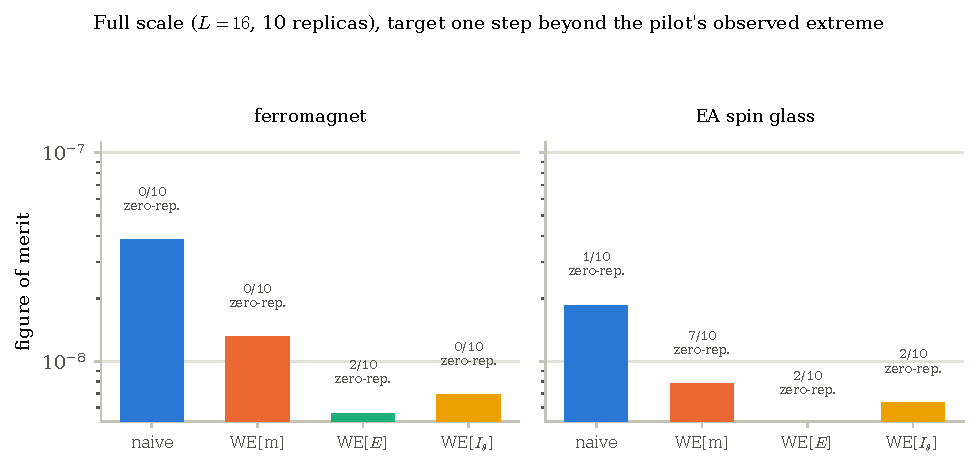
\includegraphics[width=0.92\textwidth]{figs/fig_prefix.pdf}
		\captionof{figure}{Full scale, both models: FOM by method (log scale) with zero-replica
			counts annotated, at target $|m|\ge0.9297$ (ferromagnet) and $E/N\le-1.0625$ (EA spin
			glass), 10 replicas. Bar height alone does not tell the whole story ---
			$\mathrm{WE}[E]$ has the fewest zero-replicas of any weight-window method on the
			ferromagnet but a middling FOM, which is why both numbers are reported together.}
		\label{fig:prefix}
	\end{minipage}
	\par\vspace{0.8\baselineskip}
	
	Two readings are needed. Naive Monte Carlo wins on raw FOM in both models at this rarity
	($\sim\!4\times10^{-5}$); and on the spin glass, with $\mathrm{WE}[E]$ and
	$\mathrm{WE}[I_\theta]$ on equal footing (both 2/10 zero-replicas), \textbf{the learned
		coordinate has the higher FOM by $\sim$27\%} ($6.36\times10^{-9}$ vs.\
	$5.00\times10^{-9}$) --- the first apples-to-apples advantage for the learned coordinate
	over the best hand-picked one, and the direct predecessor of the milestoning result below.
	$\mathrm{WE}[m]$ fails in most spin-glass replicas (7/10), confirming that magnetization
	carries essentially no information about this landscape.
	
	That the learned coordinate is not merely a noisy copy of energy is confirmed by a separate
	diagnostic, which regresses the rare-event label on energy alone, on $I_\theta$ alone, and
	on both, at matched training budget (Table~\ref{tab:diagnostic}). The incremental $R^2$ of
	$+0.250$ is far above the diagnostic's own noise threshold ($0.02$): $I_\theta$ carries
	substantial genuine information about the spin glass that energy alone does not have,
	consistent with the FOM advantage measured directly in Fig.~\ref{fig:prefix}.
	
	% --- TABLE 1 ---
	\begin{table}[H]
		\centering\small
		\caption{Incremental-$R^2$ diagnostic, EA spin glass, $L=16$, matched training budget
			(MSE $1.0\to0.271$ over 20 epochs).}
		\label{tab:diagnostic}
		\begin{tabular}{lr}
			\toprule
			Quantity & value \\
			\midrule
			Pearson corr$(I_\theta,\,E/N)$ & $-0.614$ \\
			fraction of $\mathrm{Var}(I_\theta)$ unexplained by $E/N$ & $0.623$ \\
			$R^2(\text{label}\sim E/N\text{ alone})$ & $0.358$ \\
			$R^2(\text{label}\sim I_\theta\text{ alone})$ & $0.577$ \\
			$R^2(\text{label}\sim E/N+I_\theta)$ & $0.608$ \\
			\textbf{incremental $R^2$ from $I_\theta$ beyond $E/N$} & $\mathbf{+0.250}$ \\
			\bottomrule
		\end{tabular}
	\end{table}
	
	Simply pushing the target rarer does not settle the naive-versus-learned comparison.
	Rerunning one threshold step deeper leaves 4--10 of 10 replicas failing across every method,
	including naive itself (4/10, versus 1/10 at the shallower target), so the resulting numbers
	are noise over noise rather than a result. This run established the ladder-difficulty
	discipline of \S\ref{sec:methods} for the remainder of the project, and motivated the
	milestoning objective below --- a change to the training label rather than to the
	weight-window schedule.
	
	\subsection{Milestoning labels: a clean regime, but strong seed dependence}\label{sec:milestone}
	On the EA spin glass at $L=16$, one threshold step beyond the pilot's observed extreme
	(``beyond=1''), every method reaches \textbf{0/10 zero-replicas} --- the cleanest,
	most-trustworthy regime obtained in this project by the ladder-difficulty standard
	(Table~\ref{tab:milestone}).
	
	% --- TABLE 2 ---
	\begin{table}[H]
		\centering\small
		\caption{Reference methods, EA spin glass, $L=16$, $T=2.6$, one step beyond the pilot
			extreme, 10 replicas, milestoning labels. All three are bit-identical across every
			training run, since none depends on the trained network. The corresponding
			$\mathrm{WE}[I_\theta]$ results --- eighteen independent runs of the identical
			configuration, seventeen with per-replica data retained --- are shown individually in
			Fig.~\ref{fig:seedsweep}; seed 0 was run twice and reproduced bit-for-bit.}
		\label{tab:milestone}
		\begin{tabular}{lrrrr}
			\toprule
			Method & $\hat\pi$ & rel.\ s.d.\ & FOM & zero-replicas \\
			\midrule
			naive & $5.29\times10^{-5}$ & 0.225 & $\mathbf{1.48\times10^{-7}}$ & 0/10 \\
			$\mathrm{WE}[m]$ & $5.55\times10^{-5}$ & 0.201 & $1.17\times10^{-7}$ & 0/10 \\
			$\mathrm{WE}[E]$ & $4.49\times10^{-5}$ & 0.209 & $4.22\times10^{-8}$ & 0/10 \\
			\bottomrule
		\end{tabular}
	\end{table}
	
	Every $\mathrm{WE}[I_\theta]$ run is, as far as the pipeline is concerned, the \emph{same
		experiment}: identical target, identical training data from cached labels, identical
	hyperparameters. The only thing that varies is the network's random weight initialization
	(\texttt{torch.manual\_seed} was absent from this driver; found and fixed during this
	investigation, then swept explicitly via \texttt{--net-seed}). \textbf{Seventeen seeds give
		seventeen different outcomes, ranging from a $52\%$ loss to a $112\%$ win against
		$\mathrm{WE}[E]$} --- a wide, roughly symmetric spread around a small positive average.
	The seeding fix is complete: seed 0 was run twice and reproduced bit-for-bit, including the
	full 1774--1776\,s wall-clock trajectory, ruling out any other unseeded source of variation.
	
	Pooling the seventeen with a two-level bootstrap --- outer resample over seeds, inner
	resample over each seed's 10 replicas --- gives a geometric-mean FOM ratio of $1.19\times$
	with 95\% CI $[0.84, 1.75]$ (median-of-ratios agrees: $1.20\times$, CI $[0.74, 1.85]$; the
	arithmetic mean of ratios is unstable at $R=10$, because bootstrap draws landing on
	near-duplicate resamples give rel.\ s.d.\ near zero and, since
	$\mathrm{FOM}\propto1/\mathrm{rel.\,var.}$, produce large outliers). Tracked at four
	checkpoints as seeds were added --- $1.28\times$ ($n=7$), $1.17\times$ ($n=9$),
	$1.28\times$ ($n=12$), $1.19\times$ ($n=17$) --- the estimate does \emph{not} trend in
	either direction; what moves monotonically is the CI width ($1.73\to1.36\to1.18\to0.91$),
	the expected signature of averaging down noise around a small effect whose sign is not
	resolved by seed count alone. Figure~\ref{fig:seedsweep} shows both the per-seed spread and the checkpoint trajectory.
	Naive Monte Carlo has the best raw FOM in every run at this
	rarity ($\sim\!5\times10^{-5}$) regardless of seed, the same lesson demonstrated in
	miniature by the 1D toy walk of \S\ref{sec:validation}.
	
	% --- FIGURE 3 ---
	\noindent
	\begin{minipage}{\linewidth}
		\centering
		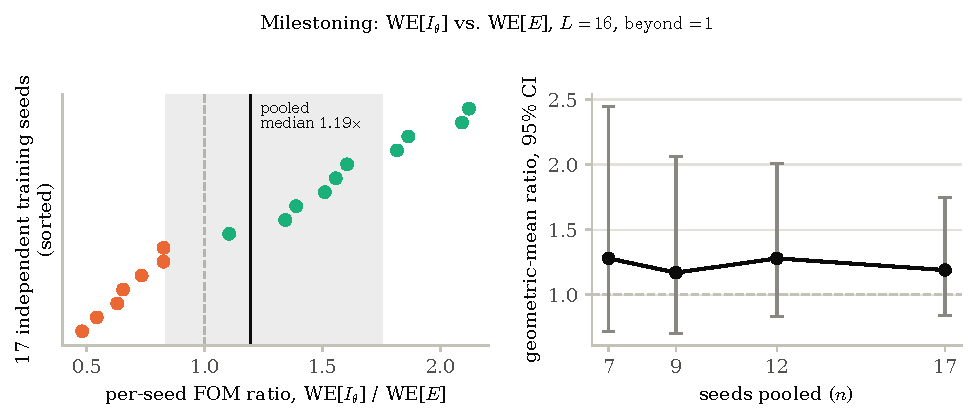
\includegraphics[width=0.92\textwidth]{figs/fig_seed_sweep.pdf}
		\captionof{figure}{Left: all 17 per-seed FOM ratios (sorted), with the pooled two-level-bootstrap
			median and 95\% CI shaded. Right: the four tracked checkpoints as seeds were added ---
			the point estimate bounces while the CI width shrinks monotonically, the expected
			signature of averaging down noise around a small, sign-unresolved effect.}
		\label{fig:seedsweep}
	\end{minipage}
	\par\vspace{0.8\baselineskip}
	
	A plausible infrastructure explanation for the spread was tested and ruled out. One
	candidate cause is that $\mathrm{WE}[I_\theta]$'s bin range was left adaptive (auto-ranging
	from the population actually explored) rather than calibrated to the coordinate's own
	scale, unlike $\mathrm{WE}[E]$ and $\mathrm{WE}[m]$. Two calibrations were tried: a
	theoretical one from the label's own z-score normalization, verified \emph{before} spending
	compute on it to be wrong (the network's real output never approaches those extremes, since
	training MSE never reaches 0); and an empirical one, from what each trained network actually
	outputs on the pilot population and training set. Run head-to-head against the untouched
	adaptive baseline on matched net-seeds (identical trained network per pair, only the bin
	range differing), the empirical calibration made both the mean FOM ratio
	($0.79\times\to0.61\times$) and the rel.\ s.d.\ ($0.214\to0.286$) \emph{worse} across seeds
	1--3. A fixed range clips any walker that exceeds it into the boundary bin, while adaptive
	tracking never does; for a coordinate whose true dynamic range over a multi-thousand-iteration
	WE trajectory is not well estimated from a static pre-run snapshot, that clipping costs more
	resolution than the calibration gains. The seed variance is therefore intrinsic to what each
	trained network learns, not an artifact of how its output is binned.
	
	Bin-count tuning is likewise ruled out as a fix. One threshold step rarer
	(Table~\ref{tab:milestone2}), $\mathrm{WE}[I_\theta]$ scores worse than $\mathrm{WE}[E]$ in
	every configuration tried: at the default bin count, at double the replica count
	($R=10\to20$, same $n_{\rm bins}=50$, same qualitative pattern), and at a $1.8\times$ larger
	bin count ($n_{\rm bins}=50\to90$), which made $\mathrm{WE}[I_\theta]$'s \emph{own} FOM
	worse rather than better ($8.36\times10^{-9}\to5.36\times10^{-9}$). A genuine resolution
	shortfall would improve with more bins, not degrade. The mechanism is structural: the
	learned coordinate's walker-population cost scales with bin count, while a discretized
	coordinate like energy naturally saturates a small, fixed number of bins and does not pay
	that overhead as it grows.
	
	% --- TABLE 3 ---
	\begin{table}[H]
		\centering\small
		\caption{EA spin glass, $L=16$, one step rarer than Table~\ref{tab:milestone}, milestoning
			labels, default configuration ($n_{\rm bins}=50$, $R=10$).}
		\label{tab:milestone2}
		\begin{tabular}{lrr}
			\toprule
			Method & FOM & zero-rep.\ \\
			\midrule
			naive & $3.51\times10^{-8}$ & 0/10 \\
			$\mathrm{WE}[m]$ & $7.73\times10^{-9}$ & 0/10 \\
			$\mathrm{WE}[E]$ & $9.21\times10^{-9}$ & 0/10 \\
			$\mathrm{WE}[I_\theta]$ & $8.36\times10^{-9}$ & 0/10 \\
			\bottomrule
		\end{tabular}
	\end{table}
	
	\subsubsection{Deep ensembling: the seed variance is reducible, but converges to a loss}
	\label{sec:ensemble}
	Table~\ref{tab:milestone} leaves one question to settle: is the seed-to-seed spread genuine
	noise around a real advantage, or is the positive point estimate itself an artifact of a few
	lucky initializations? Rather than add more single-net seeds --- already shown not to close
	the CI at reasonable cost --- we attacked the diagnosed noise source directly.
	\texttt{run\_milestone.py} was extended with \texttt{--ensemble K}: train $K$
	independently-initialized networks on the identical milestone labels and use their
	\emph{mean} prediction as $I_\theta$, a standard deep-ensemble variance-reduction step.
	$K=1$ reproduces the original single-net code path exactly (verified bit-identical output on
	a smoke config). Five independent ensembles ($K=5$ each, base seeds 20--24) were run at the
	identical configuration as Table~\ref{tab:milestone} (beyond$=1$, $\tau=2$, $R=10$).
	
	% --- TABLE 4 ---
	\begin{table}[H]
		\centering\small
		\caption{Five independent $K{=}5$ deep-ensemble runs, identical configuration to
			Table~\ref{tab:milestone}. FOM ratio is $\mathrm{WE}[I_\theta]/\mathrm{WE}[E]$ on the
			MC-sweep cost as originally defined.}
		\label{tab:ensemble}
		\begin{tabular}{lrrr}
			\toprule
			Run & $\mathrm{WE}[I_\theta]$ FOM & rel.\ s.d.\ & ratio vs.\ $\mathrm{WE}[E]$ \\
			\midrule
			ensemble, base seed 20 & $1.95\times10^{-8}$ & 0.272 & $0.46\times$ ($-54\%$) \\
			ensemble, base seed 21 & $2.75\times10^{-8}$ & 0.229 & $0.65\times$ ($-35\%$) \\
			ensemble, base seed 22 & $3.69\times10^{-8}$ & 0.199 & $0.88\times$ ($-12\%$) \\
			ensemble, base seed 23 & $3.07\times10^{-8}$ & 0.215 & $0.73\times$ ($-27\%$) \\
			ensemble, base seed 24 & $3.84\times10^{-8}$ & 0.194 & $0.91\times$ ($-9\%$) \\
			\bottomrule
		\end{tabular}
	\end{table}
	
	Two findings follow, both against the ensemble. \textbf{First}, ensembling did what it was
	supposed to do to the \emph{variance}: the five ratios of Table~\ref{tab:ensemble} span $0.46$--$0.91\times$, far
	tighter than the seventeen single-net seeds' $-52\%$ to $+112\%$ spread. But the value it
	converges toward is a loss, not the earlier $\sim\!1.2\times$ point estimate: a two-level
	bootstrap (outer over the 5 runs, inner over each run's 10 replicas, identical machinery to
	Table~\ref{tab:milestone}) gives a geometric-mean ratio of $0.74\times$, 95\% CI
	$[0.43, 1.32]$ --- not significant, but on the opposite side of 1 from the single-net pooled
	estimate. Read together, the most consistent interpretation is that the single-net sweep's
	more extreme positive draws ($+82\%, +109\%, +112\%$) were high-variance artifacts of
	individual weight initializations rather than signal, and $I_\theta$'s true expected
	performance is at or below $\mathrm{WE}[E]$'s.
	
	\textbf{Second, and decisive}, the ensemble exposed a cost-accounting bug that applies to
	every $\mathrm{WE}[I_\theta]$ result in this paper, though it is negligible at $K=1$.
	\texttt{we\_estimate()}'s \texttt{cost} field counts Monte Carlo sweeps only
	($|S|\cdot\tau\cdot L^2$) and is blind to neural-network inference. At $K=1$ a single
	forward pass is cheap enough relative to the MC cost that the omission does not matter; at
	$K=5$ it does. Measured directly from wall-clock timestamps rather than the MC-cost field,
	$\mathrm{WE}[I_\theta]$ took $10.7$--$10.9\times$ $\mathrm{WE}[E]$'s wall-clock time in
	every one of the five runs --- remarkably consistent --- while the MC-cost field implied
	only $\sim\!1.3\times$. Recomputing FOM with measured wall-clock cost, using the same
	bootstrap, gives a geometric-mean ratio of $0.087\times$, 95\% CI $[0.051, 0.155]$: the only
	comparison in this paper whose confidence interval \emph{excludes} 1.0 in either direction.
	\texttt{run\_milestone.py} now records measured \texttt{wall\_time} per method, so the
	correction no longer requires post-hoc log parsing.
	
	Deep ensembling therefore does not rescue the learned coordinate. It reduces run-to-run
	variance exactly as a deep ensemble should, but converges to a value at or below parity with
	the hand-picked energy coordinate, and once its real inference cost is counted at all the
	comparison is a decisive, statistically significant loss.
	
	\subsection{The self-consistency objective of Kim and Cai}\label{sec:kimcai}
	The self-consistency training objective of \S\ref{sec:objectives} was implemented, gated
	against exact enumeration at $L=4$ (learned-coordinate unbiasedness ratio 1.004), and run
	head-to-head against the surrogate objective, first at laptop scale and then at full scale.
	At $L=12$ and the shallowest calibrated target, the self-consistency objective's point
	estimate already exceeded the surrogate's ($4.98\times10^{-8}$ vs.\ $2.93\times10^{-8}$,
	with fewer zero-replicas, 2/6 vs.\ 3/6), though it still fell short of $\mathrm{WE}[E]$'s
	$7.53\times10^{-8}$ at this rarity. Its training cost is real even here:
	$\sim$94$\times$ longer than the surrogate objective at this scale ($\sim$752\,s vs.\
	$\sim$8\,s), from the additional $N=L^2$ network evaluations the self-consistency loss
	requires per training configuration.
	
	At full scale ($L=16$) and the shallowest calibrated target --- ``beyond''\,$=0$, the
	easiest regime, in which every method reaches 0--1 zero-replicas out of 10 --- the
	self-consistency coordinate's \emph{point estimate} exceeds both the hand-picked energy
	coordinate and this project's own surrogate coordinate (Table~\ref{tab:kimcai}).
	
	% --- TABLE 5 ---
	\begin{table}[H]
		\centering\small
		\caption{EA spin glass, $L=16$, shallowest calibrated target, 10 replicas. Point estimates
			only --- see the bootstrapped intervals in Fig.~\ref{fig:kimcai}.}
		\label{tab:kimcai}
		\begin{tabular}{lrrrr}
			\toprule
			Method & $\hat\pi$ & rel.\ s.d.\ & FOM & zero-replicas \\
			\midrule
			naive & $3.36\times10^{-5}$ & 0.294 & $8.60\times10^{-8}$ & 0/10 \\
			$\mathrm{WE}[m]$ & $3.94\times10^{-5}$ & 0.553 & $8.81\times10^{-8}$ & 1/10 \\
			$\mathrm{WE}[E]$ & $3.39\times10^{-5}$ & 0.671 & $1.33\times10^{-8}$ & 0/10 \\
			$\mathrm{WE}[I_\theta]$ surrogate & $2.92\times10^{-5}$ & 0.904 & $8.62\times10^{-9}$ & 1/10 \\
			$\mathrm{WE}[I_\theta]$ self-consistent & $4.01\times10^{-5}$ & 0.655 &
			$1.62\times10^{-8}$ & 0/10 \\
			\bottomrule
		\end{tabular}
	\end{table}
	
	That point estimate does not survive a bootstrap check, and the effect shrinks under
	replication. Both configurations were re-run with per-replica values retained, and the FOM
	ratio between methods bootstrapped by resampling the replica axis independently for each
	side --- no shared random-number seed to pair on, since uniform-style and biased allocations
	consume different numbers of walkers per bin and desynchronise almost immediately, the same
	obstruction encountered independently in the FW-CADIS common-random-numbers attempt of
	\S\ref{sec:fwcadis}. Because training here is a fixed cost independent of replica count (a
	deterministic seed; only the cheap evaluation step scales with $R$), tripling to $R=30$ cost
	roughly six additional minutes on top of the $\sim$76-minute training already paid.
	Figure~\ref{fig:kimcai} reports the result, together with the same comparison run one
	threshold step deeper (depth 1, the depth of Table~\ref{tab:milestone}), where the
	zero-replica counts are 2/10 for the surrogate against 1/10 for the self-consistent
	objective.
	
	No ratio is significant at any depth or replica count. At $R=30$ both confidence intervals
	tighten substantially \emph{and} both median ratios move toward 1 --- against the surrogate
	from $1.83\times$ ($[0.49,\,9.23]$) to $1.39\times$ ($[0.65,\,2.95]$), and against
	$\mathrm{WE}[E]$ from $1.19\times$ ($[0.33,\,4.95]$) to $1.07\times$ ($[0.55,\,2.09]$) --- not merely a
	tightening interval around the original estimate, but the point estimate itself receding,
	which we read as evidence that the original $R=10$ advantage was substantially noise. The
	deeper target tells the same story from the other direction: the point-estimate gap versus
	the surrogate \emph{shrank} ($1.83\times\to1.14\times$) rather than growing, even as the
	self-consistency coordinate kept its relative reliability advantage (fewest zero-replicas of
	any weight-window method at both depths). One more noisy $R=10$ point estimate does not
	resolve the depth question either way, but it does rule out the simplest optimistic story,
	that the advantage would obviously grow once naive and the surrogate objective start to
	struggle.
	
	% --- FIGURE 4 ---
	\noindent
	\begin{minipage}{\linewidth}
		\centering
		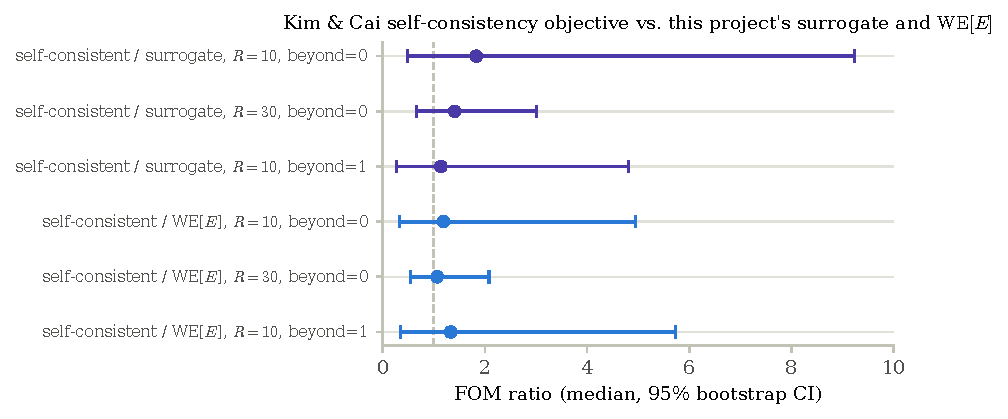
\includegraphics[width=0.85\textwidth]{figs/fig_kimcai.pdf}
		\captionof{figure}{Bootstrapped FOM ratios, full scale ($L=16$), as a forest plot: the
			self-consistency objective against the surrogate objective and against
			$\mathrm{WE}[E]$, at depth 0 ($R=10$ and $R=30$) and depth 1 ($R=10$). A ratio above 1
			favors the self-consistency objective. Every interval crosses the ratio-1 reference
			line (dashed); the $R{=}30$ intervals (recomputed directly from the retained
			per-replica arrays via the same replica-resampling bootstrap) are visibly tighter than
			their $R{=}10$ counterparts without the median crossing to the other side of 1.}
		\label{fig:kimcai}
	\end{minipage}
	\par\vspace{0.8\baselineskip}
	
	In summary, the self-consistency-trained coordinate is the most reliable weight-window
	method tested in every regime examined, and its point estimate is consistently the best of
	the learned-coordinate variants, but a quantified FOM advantage over this project's own
	surrogate objective is not established at any depth or replica count tested and shows no
	sign of strengthening with depth. It is also markedly more expensive to train: roughly
	$170\times$ slower per epoch than the surrogate objective at full scale ($\sim$76 minutes
	versus $\sim$4).
	
	\subsection{Lattice-size dependence of naive dominance}\label{sec:lscaling}
	Both \S\ref{sec:res-learned} and \S\ref{sec:milestone} find naive Monte Carlo winning on raw
	FOM at $L=16$. This is better read as a finite-size effect than as a failure of variance
	reduction. Naive's cost is fixed by the replica budget (naive\_chains $\times$ naive\_sweeps
	in our runs) independent of the target's rarity $\pi$, while its relative variance grows as
	$\pi$ shrinks; WE's cost is likewise fixed by its own budget
	($n_{\rm bins}\times n_{\rm per\ bin}\times\mathrm{we\_iter}$), but once it penetrates to
	the target its relative variance is largely rarity-independent. The two cost curves must
	cross somewhere, and at a rarity shallow enough for naive to sample the event comfortably,
	naive wins almost by construction, since WE pays a penetration overhead the problem does not
	yet need. We tested this directly with a lattice-size scan at fixed $T=2.6$,
	$\mathrm{beyond}=1$, $\tau=2$: $L\in\{8,16,24,32\}$, with naive\_chains/naive\_sweeps held
	fixed across all four so that naive's cost is genuinely $L$-independent as the argument
	requires (Fig.~\ref{fig:lscaling}).
	
	\textbf{Naive wins at every tested $L$, and the margin does not shrink --- if anything it
		grows slightly and then plateaus, from $1.9\times$ at $L=8$ to $\sim\!3.5\times$ by
		$L=16$ and beyond.} This holds across nearly five orders of magnitude of target rarity
	($\hat\pi$ from $1.8\times10^{-4}$ down to $4.2\times10^{-6}$) and is robust to which WE
	variant is best at a given $L$ (the winner changes: $\mathrm{WE}[E]$ at $L=8,24$,
	$\mathrm{WE}[m]$ at $L=16$, $\mathrm{WE}[I_\theta]$ at $L=32$). Within the range tested
	there is no sign of the naive/WE crossover opening as $L$ grows; if it exists at all on this
	problem, it lies beyond $L=32$ at this temperature. The precise claim supported here is
	therefore narrower than ``variance reduction does not pay off'': it is that no tested rarity
	was found, at any $L$ up to 32, at which naive fails to converge while a WE-based method
	succeeds.
	
	% --- FIGURE 5 ---
	\noindent
	\begin{minipage}{\linewidth}
		\centering
		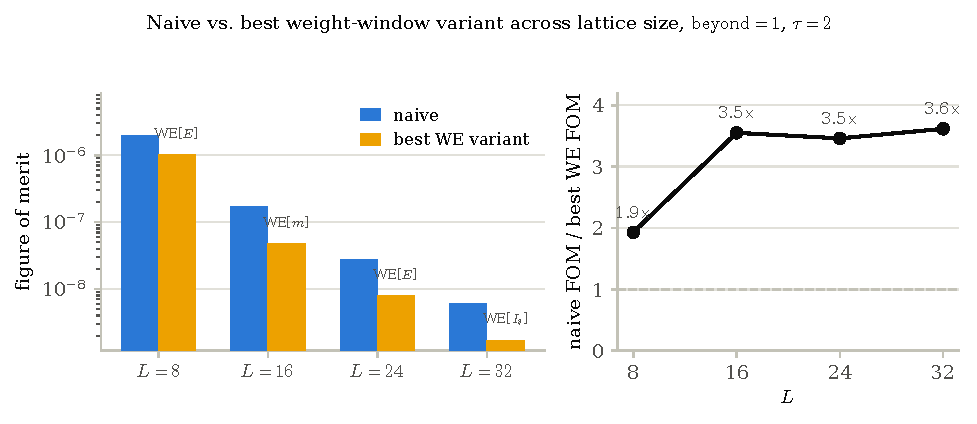
\includegraphics[width=0.92\textwidth]{figs/fig_lscaling.pdf}
		\captionof{figure}{Lattice-size scan, EA spin glass, $\mathrm{beyond}=1$, $T=2.6$,
			$\tau=2$. Left: naive vs.\ the best-performing WE variant at each $L$, FOM on a log
			scale, labeled with which variant won; naive's $\hat\pi$ falls from
			$1.79\times10^{-4}$ at $L=8$ to $4.17\times10^{-6}$ at $L=32$. Right: the ratio
			itself --- it opens from $L=8$ to $L=16$ and then plateaus around $3.5\times$, with no
			sign of narrowing back toward the naive/WE crossover within the tested range.}
		\label{fig:lscaling}
	\end{minipage}
	\par\vspace{0.8\baselineskip}
	
	One secondary pattern is visible but reported only as a point estimate:
	$\mathrm{WE}[I_\theta]$ is the weakest WE variant at $L=8,16,24$ but the \emph{strongest} at
	$L=32$, consistent with a learned coordinate's advantage over hand-picked ones mattering
	more as the landscape gets harder. We do not treat this as established, because the
	milestoning network's training is not seeded in this scan, so each $\mathrm{WE}[I_\theta]$
	point in Fig.~\ref{fig:lscaling} is a single random draw from an uncharacterized
	distribution over training outcomes. The tested range also has a clear upper edge: at
	$L=40$, naive itself fails in 10 of 12 replicas, with $\mathrm{WE}[m]$ (11/12) and
	$\mathrm{WE}[E]$ (10/12) failing similarly badly, so by the ladder-difficulty discipline of
	\S\ref{sec:methods} that size is not a trustworthy comparison as run and is not reported as
	a fifth point.
	
	\subsection{FW-CADIS global allocation: cost advantage without flattening}\label{sec:fwcadis}
	The implementation is gated clean against exact enumeration at $L=4$ for both allocation
	settings, every threshold, both models: ratios of 0.999--0.998--0.989 (uniform) and
	1.005--1.012--0.992 (FW-CADIS, $\alpha=1$) on the ferromagnet, and 1.009--1.004--1.007 /
	0.986--0.980--0.983 on the spin glass, all within $\sim$2\% of exact --- confirming that all
	thresholds are correctly tallied from a single run regardless of allocation, the core
	mechanic the whole method depends on.
	
	At laptop scale ($L=12$, $R=6$, 6 thresholds) the sweep over $\alpha$ produced a
	real-looking win: $\alpha=0.25$ was the only setting with full 6/6 coverage and better
	flatness than uniform, a modest $\sim$14\% improvement ($283.8\to245.2$ in max/min relative
	error) at $\sim$2.6$\times$ lower cost. Larger $\alpha$ looked dramatically flatter but was
	disqualified by the coverage-first rule of \S\ref{sec:methods}, having stopped observing the
	deepest threshold at all. \textbf{The identical sweep at full scale reverses that finding}
	(Table~\ref{tab:fwfull}).
	
	% --- TABLE 6 ---
	\begin{table}[H]
		\centering\small
		\caption{EA spin glass, $L=16$, full preset, $R=30$, 6 thresholds spanning progress
			$0.691\to1.063$. Every allocation reaches full 6/6 coverage at this scale.}
		\label{tab:fwfull}
		\begin{tabular}{lrr}
			\toprule
			Allocation & flatness (max/min) & cost \\
			\midrule
			uniform ($\alpha=0$) & \textbf{298.0 (best)} & $1.55\times10^{8}$ \\
			$\alpha=0.25$ & 377.8 & $7.89\times10^{7}$ \\
			$\alpha=0.5$ & 323.9 & $2.35\times10^{7}$ \\
			$\alpha=0.75$ & 342.4 & $1.98\times10^{7}$ \\
			$\alpha=1.0$ & 385.5 & $1.94\times10^{7}$ ($\sim\!8\times$ cheaper) \\
			naive (reference) & 445.1 & $1.34\times10^{8}$ \\
			\bottomrule
		\end{tabular}
	\end{table}
	
	At full scale \emph{every} tested $\alpha$ is worse than uniform on flatness, and not even
	monotonic in $\alpha$ among the FW-CADIS runs ($\alpha=0.5$ beats both $0.25$ and $1.0$).
	All are substantially cheaper (2--8$\times$), so the method is not doing nothing, but it is
	not delivering the flattening it exists to demonstrate at this lattice size, bin count, and
	threshold spacing. Every remaining lever was then tried against that finding: bootstrap
	confidence intervals on the flatness metric; a replica increase from $R=30$ to $R=90$;
	wiring the learned coordinate of \S\ref{sec:milestone} in as the FW-CADIS binning axis
	instead of the physical progress coordinate (gated clean at $L=4$, tested at scale: no
	improvement, roughly double the cost); a common-random-numbers paired-difference design,
	which does \emph{not} engage on this problem (correlation between the two allocations'
	same-seed estimates measured $\approx-0.05$ to $-0.10$, essentially zero, because the two
	allocations consume different numbers of walkers per bin and desynchronise the random stream
	almost immediately after the first resampling step); and laddering the threshold family to
	its shallowest calibrated depth, combined with the larger replica count. The most favorable
	configuration reached is Table~\ref{tab:fwcadis}.
	
	% --- TABLE 7 ---
	\begin{table}[H]
		\centering\small
		\caption{EA spin glass, $L=16$, shallowest calibrated threshold family, $R=90$: the final,
			most favorable configuration tested for FW-CADIS.}
		\label{tab:fwcadis}
		\begin{tabular}{lrrr}
			\toprule
			Allocation & flatness (max/min) & 95\% CI & cost \\
			\midrule
			Uniform ($\alpha=0$) & 276.1 & $[224,\,344]$ & $1.59\times10^{8}$ \\
			FW-CADIS ($\alpha=1$) & 297.3 & $[234,\,388]$ & $1.99\times10^{7}$ ($\mathbf{\sim\!8\times}$ \textbf{cheaper}) \\
			\bottomrule
		\end{tabular}
	\end{table}
	
	The two confidence intervals overlap, and the paired-difference estimate is $+20.9$ with
	95\% CI $[-77.2,\,+137.6]$, also including zero. Across every $\alpha$, replica count, and
	coordinate tried, the point-estimate \emph{direction} consistently favored uniform
	allocation over FW-CADIS on raw flatness, never the reverse. The confidence-interval width
	scaled almost exactly as $1/\sqrt{R}$ between $R=30$ and $R=90$ (predicted shrink factor
	0.577, observed 0.597); extrapolating that scaling, fully resolving the residual gap would
	need on the order of $R\approx2300$ replicas, and given the consistent direction such a run
	would most likely confirm uniform allocation as measurably flatter rather than produce a win
	for FW-CADIS. \textbf{The result we report is therefore that on this problem FW-CADIS does
		not measurably flatten relative error across a threshold family better than uniform
		allocation, but achieves a statistically indistinguishable error profile at approximately
		one-eighth the simulation cost.} The cost advantage is real and reproducible; the
	flattening advantage the method is named for is the part that did not materialize.
	
	This is not a property of the adversarial spin-glass landscape. Repeating the identical
	comparison on the ferromagnet, where the reaction coordinate is known to be good and the
	equilibrium landscape smooth (Table~\ref{tab:fwferro}), the two confidence intervals do
	\emph{not} overlap: the paired-difference estimate is $+178.2$ with 95\% CI
	$[+59.8,\,+351.3]$, excluding zero. \textbf{On the easier landscape FW-CADIS is not merely
		inconclusive but measurably, statistically confirmed \emph{worse} than uniform
		allocation} --- the opposite of what a landscape-difficulty explanation would predict,
	since the spin glass, where the method's own hypothesis says a global map should matter
	most, never reached this level of statistical resolution in either direction.
	The per-threshold error profiles behind both comparisons are shown in
	Fig.~\ref{fig:fwcadis}. Common-random-numbers correlation here measured $0.062$, consistent with zero and with the
	mechanism identified above: the two allocations consume different walker populations per bin
	regardless of which model is sampled. The explanation therefore lies in this specific
	parameterisation --- bin count, threshold spacing, or the inverse-response weighting itself
	at this scale --- rather than in spin-glass frustration.
	
	% --- TABLE 8 ---
	\begin{table}[H]
		\centering\small
		\caption{Ferromagnet, $L=16$, shallowest calibrated threshold family, $R=30$ --- the
			landscape where the coordinate is known-good, unlike the spin glass used everywhere else
			in this section.}
		\label{tab:fwferro}
		\begin{tabular}{lrrr}
			\toprule
			Allocation & flatness (max/min) & 95\% CI & cost \\
			\midrule
			Uniform ($\alpha=0$) & \textbf{100.9} & $[65.8,\,160.3]$ & $1.96\times10^{8}$ \\
			FW-CADIS ($\alpha=1$) & 287.3 & $[194.7,\,414.8]$ & $3.09\times10^{7}$ \\
			\bottomrule
		\end{tabular}
	\end{table}
	
	% --- FIGURE 6 ---
	\noindent
	\begin{minipage}{\linewidth}
		\centering
		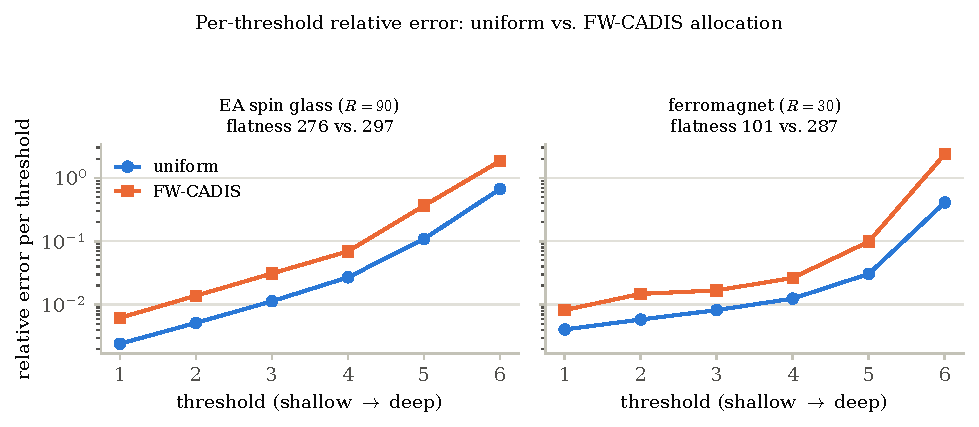
\includegraphics[width=0.92\textwidth]{figs/fig_fwcadis.pdf}
		\captionof{figure}{Per-threshold relative error (log scale), uniform vs.\ FW-CADIS allocation, at
			the final tested configuration for each model (Table~\ref{tab:fwcadis} spin glass,
			Table~\ref{tab:fwferro} ferromagnet). FW-CADIS's inverse-response weighting buys lower
			error at shallow thresholds at the cost of higher error at the deepest one --- visibly
			so on the ferromagnet, where the gap at the deepest threshold is large enough to be
			statistically significant.}
		\label{fig:fwcadis}
	\end{minipage}
	\par\vspace{0.8\baselineskip}
	
	\FloatBarrier
	
	% ========================================================================
	\section{Conclusions}\label{sec:conclusions}
	The transport--statistical-mechanics correspondence this project set out to test is real
	where it can be proved. The adjoint$=$committor identity is exact, tilting by the exact
	committor is provably zero-variance and was confirmed numerically to $\sim\!10^{-30}$
	relative variance on a solvable toy walk, and Weighted Ensemble --- weight windows applied
	to spin configurations --- reproduces exact enumeration at $L=4$ to 1--2\% while reaching
	about two decades deeper into a magnetization tail than naive Monte Carlo at matched cost.
	The more experimentally demanding claims built on top of that foundation did not hold up as
	cleanly. The learned coordinate trained on milestoned committor labels does not beat the
	hand-picked energy coordinate: a deep-ensemble follow-up, designed to resolve the single-net
	seed sweep's ambiguous $1.19\times$ point estimate by attacking its diagnosed cause, settled
	it in the negative at $0.087\times$ (95\% CI $[0.051,0.155]$) on a corrected cost
	accounting, the only bootstrap interval in this paper that excludes parity. FW-CADIS
	delivers a real, reproducible cost advantage of roughly $8\times$ but not the flattening it
	is named for, on either landscape. The self-consistency objective is the most reliable
	weight-window method tested but shows no quantified FOM advantage that survives replication.
	Naive Monte Carlo's dominance over every tested weight-window variant, meanwhile, is the one
	claim that grew \emph{more} confident under additional scrutiny, holding across a four-point
	lattice-size scan up to $L=32$ with no sign of narrowing.
	
	The clearest methodological lesson of this paper is not any single number: it is that
	``0/10 zero-replicas'' and a tidy point-estimate table are not, by themselves, evidence of a
	real effect. The FW-CADIS flattening claim and the Kim \& Cai comparison both needed a
	bootstrap confidence interval to reveal that their apparent wins were noise. The milestoning
	result needed something no amount of replica-axis bootstrapping within a single run could
	have caught --- independently-trained networks --- and even the most striking of the
	seventeen point estimates ($+112\%$) turned out to sit inside a two-level bootstrap interval
	that includes 1. What finally resolved that question was not more of the same axis but a
	different one: a deep ensemble that reduced the seed-to-seed spread as a variance-reduction
	technique should, converged at or below parity, and in the course of being built fairly
	surfaced a cost-accounting bug whose correction turned a marginal-looking loss into a
	decisive one. That a genuinely decisive answer came from fixing what was being measured,
	rather than from sampling harder along an axis already shown not to help, is the most
	transferable lesson here. Reaching these conclusions required diagnosing and correcting real
	implementation issues along the way --- a resampling interval that silently degenerated a
	weight-window method to naive sampling, a mis-calibrated bin range, an under-determined
	training objective that could converge to a useless constant solution while reporting a
	plausible loss, and an unseeded network initialization that let one training run's outcome
	be mistaken for a stable result --- each caught by an independent cross-check rather than by
	a number simply looking wrong.
	
	\section*{Acknowledgements}
	The author gratefully acknowledges the support provided by Fahad Bin Sultan University, Tabuk, Saudi Arabia, for providing a supportive academic environment and access to the computational facilities necessary to conduct this research. The institutional support and research infrastructure offered by the university were essential for implementing the Monte Carlo experiments and performing the systematic statistical analysis reported in this work.
	
	% To print the CRediT authorship contribution details
	\printcredits
	
	%% Bibliography (manual list, ordered by first citation)
	\begin{thebibliography}{99}
		
		\bibitem{allen2009}
		R. J. Allen, C. Valeriani, and P. R. ten Wolde, ``Forward flux sampling for rare event simulations,'' \emph{Journal of Physics: Condensed Matter}, vol. 21, no. 46, 463102, 2009.
		
		\bibitem{zuckerman2017}
		D. M. Zuckerman and L. T. Chong, ``Weighted ensemble simulation: Review of methodology, applications, and software,'' \emph{Annual Review of Biophysics}, vol. 46, pp. 43--57, 2017.
		
		\bibitem{e2006}
		W. E and E. Vanden-Eijnden, ``Towards a theory of transition paths,'' \emph{Journal of Statistical Physics}, vol. 123, no. 3, pp. 503--523, 2006.
		
		\bibitem{touchette2009}
		H. Touchette, ``The large deviation approach to statistical mechanics,'' \emph{Physics Reports}, vol. 478, no. 1--3, pp. 1--69, 2009.
		
		\bibitem{kahn1951}
		H. Kahn and T. E. Harris, ``Estimation of particle transmission by random sampling,'' \emph{National Bureau of Standards Applied Mathematics Series}, vol. 12, pp. 27--30, 1951.
		
		\bibitem{kahn1953}
		H. Kahn and A. W. Marshall, ``Methods of reducing sample size in Monte Carlo computations,'' \emph{Journal of the Operations Research Society of America}, vol. 1, no. 5, pp. 263--278, 1953.
		
		\bibitem{spanier1969}
		J. Spanier and E. M. Gelbard, \emph{Monte Carlo Principles and Neutron Transport Problems}. Reading, MA: Addison-Wesley, 1969.
		
		\bibitem{wagner1998}
		J. C. Wagner and A. Haghighat, ``Automated variance reduction of Monte Carlo shielding calculations using the discrete ordinates adjoint function,'' \emph{Nuclear Science and Engineering}, vol. 128, no. 2, pp. 186--208, 1998.
		
		\bibitem{lewins1965}
		J. Lewins, \emph{Importance: The Adjoint Function}. Oxford: Pergamon Press, 1965.
		
		\bibitem{bell1970}
		G. I. Bell and S. Glasstone, \emph{Nuclear Reactor Theory}. New York: Van Nostrand Reinhold, 1970.
		
		\bibitem{booth1984}
		T. E. Booth and J. S. Hendricks, ``Importance estimation in forward Monte Carlo calculations,'' \emph{Nuclear Technology/Fusion}, vol. 5, p. 90, 1984.
		
		\bibitem{haghighat2003}
		A. Haghighat and J. C. Wagner, ``Monte Carlo variance reduction with deterministic importance functions,'' \emph{Progress in Nuclear Energy}, vol. 42, no. 1, pp. 25--53, 2003.
		
		\bibitem{wagnerfw2014}
		J. C. Wagner, D. E. Peplow, and S. W. Mosher, ``FW-CADIS method for global and regional variance reduction of Monte Carlo radiation transport calculations,'' \emph{Nuclear Science and Engineering}, vol. 176, no. 1, pp. 37--57, 2014.
		
		\bibitem{cooper2001}
		M. A. Cooper and E. W. Larsen, ``Automated weight windows for global Monte Carlo particle transport calculations,'' \emph{Nuclear Science and Engineering}, vol. 137, no. 1, pp. 1--13, 2001.
		
		\bibitem{metzner2009}
		P. Metzner, C. Sch\"{u}tte, and E. Vanden-Eijnden, ``Transition path theory for Markov jump processes,'' \emph{Multiscale Modeling \& Simulation}, vol. 7, no. 3, pp. 1192--1219, 2009.
		
		\bibitem{evanden2010}
		W. E and E. Vanden-Eijnden, ``Transition-path theory and path-finding algorithms for the study of rare events,'' \emph{Annual Review of Physical Chemistry}, vol. 61, pp. 391--420, 2010.
		
		\bibitem{huber1996}
		G. A. Huber and S. Kim, ``Weighted-ensemble Brownian dynamics simulations for protein association reactions,'' \emph{Biophysical Journal}, vol. 70, no. 1, pp. 97--110, 1996.
		
		\bibitem{zhang2010}
		B. W. Zhang, D. Jasnow, and D. M. Zuckerman, ``The `weighted ensemble' path sampling method is statistically exact for a broad class of stochastic processes and binning procedures,'' \emph{The Journal of Chemical Physics}, vol. 132, 054107, 2010.
		
		\bibitem{cerou2007}
		F. C\'{e}rou and A. Guyader, ``Adaptive multilevel splitting for rare event analysis,'' \emph{Stochastic Analysis and Applications}, vol. 25, no. 2, pp. 417--443, 2007.
		
		\bibitem{bolhuis2002}
		P. G. Bolhuis, D. Chandler, C. Dellago, and P. L. Geissler, ``Transition path sampling: Throwing ropes over rough mountain passes, in the dark,'' \emph{Annual Review of Physical Chemistry}, vol. 53, pp. 291--318, 2002.
		
		\bibitem{ising1925}
		E. Ising, ``Beitrag zur Theorie des Ferromagnetismus,'' \emph{Zeitschrift f\"{u}r Physik}, vol. 31, no. 1, pp. 253--258, 1925.
		
		\bibitem{onsager1944}
		L. Onsager, ``Crystal statistics. I. A two-dimensional model with an order-disorder transition,'' \emph{Physical Review}, vol. 65, no. 3--4, pp. 117--149, 1944.
		
		\bibitem{edwards1975}
		S. F. Edwards and P. W. Anderson, ``Theory of spin glasses,'' \emph{Journal of Physics F: Metal Physics}, vol. 5, no. 5, pp. 965--974, 1975.
		
		\bibitem{binder1986}
		K. Binder and A. P. Young, ``Spin glasses: Experimental facts, theoretical concepts, and open questions,'' \emph{Reviews of Modern Physics}, vol. 58, no. 4, pp. 801--976, 1986.
		
		\bibitem{metropolis1953}
		N. Metropolis, A. W. Rosenbluth, M. N. Rosenbluth, A. H. Teller, and E. Teller, ``Equation of state calculations by fast computing machines,'' \emph{The Journal of Chemical Physics}, vol. 21, no. 6, pp. 1087--1092, 1953.
		
		\bibitem{swendsen1987}
		R. H. Swendsen and J.-S. Wang, ``Nonuniversal critical dynamics in Monte Carlo simulations,'' \emph{Physical Review Letters}, vol. 58, no. 2, pp. 86--88, 1987.
		
		\bibitem{wolff1989}
		U. Wolff, ``Collective Monte Carlo updating for spin systems,'' \emph{Physical Review Letters}, vol. 62, no. 4, pp. 361--364, 1989.
		
		\bibitem{berg1992}
		B. A. Berg and T. Neuhaus, ``Multicanonical ensemble: A new approach to simulate first-order phase transitions,'' \emph{Physical Review Letters}, vol. 68, no. 1, pp. 9--12, 1992.
		
		\bibitem{wanglandau2001}
		F. Wang and D. P. Landau, ``Efficient, multiple-range random walk algorithm to calculate the density of states,'' \emph{Physical Review Letters}, vol. 86, no. 10, pp. 2050--2053, 2001.
		
		\bibitem{doob1984}
		J. L. Doob, \emph{Classical Potential Theory and Its Probabilistic Counterpart}. New York: Springer-Verlag, 1984.
		
		\bibitem{chetrite2015}
		R. Chetrite and H. Touchette, ``Nonequilibrium Markov processes conditioned on large deviations,'' \emph{Annales Henri Poincar\'{e}}, vol. 16, no. 9, pp. 2005--2057, 2015.
		
		\bibitem{hartmann2019}
		C. Hartmann, O. Kebiri, L. Neureither, and L. Richter, ``Variational approach to rare event simulation using least-squares regression,'' \emph{Chaos: An Interdisciplinary Journal of Nonlinear Science}, vol. 29, no. 6, 063107, 2019.
		
		\bibitem{raissi2019}
		M. Raissi, P. Perdikaris, and G. E. Karniadakis, ``Physics-informed neural networks: A deep learning framework for solving forward and inverse problems involving nonlinear partial differential equations,'' \emph{Journal of Computational Physics}, vol. 378, pp. 686--707, 2019.
		
		\bibitem{li2019}
		Q. Li, B. Lin, and W. Ren, ``Computing committor functions for the study of rare events using deep learning,'' \emph{The Journal of Chemical Physics}, vol. 151, no. 5, 054112, 2019.
		
		\bibitem{khoo2019}
		Y. Khoo, J. Lu, and L. Ying, ``Solving for high-dimensional committor functions using artificial neural networks,'' \emph{Research in the Mathematical Sciences}, vol. 6, no. 1, art. 1, 2019.
		
		\bibitem{rotskoff2020}
		G. M. Rotskoff, A. R. Mitchell, and E. Vanden-Eijnden, ``Active importance sampling for variational objectives dominated by rare events: Consequences for optimization and generalization,'' \emph{Proceedings of Machine Learning Research}, vol. 145, pp. 757--780, 2022.
		
		\bibitem{trizio2025}
		E. Trizio, P. Kang, and M. Parrinello, ``Everything everywhere all at once: a probability-based enhanced sampling approach to rare events,'' \emph{Nature Computational Science}, 2025; see also E. Trizio, G. Rossi, and M. Parrinello, ``Ceci n'est pas un committor, yet it samples like one: efficient sampling via approximated committor functions,'' arXiv:2602.23236, 2026.
		
		\bibitem{wu2019}
		D. Wu, L. Wang, and P. Zhang, ``Solving statistical mechanics using variational autoregressive networks,'' \emph{Physical Review Letters}, vol. 122, 080602, 2019.
		
		\bibitem{noe2019}
		F. No\'{e}, S. Olsson, J. K\"{o}hler, and H. Wu, ``Boltzmann generators: Sampling equilibrium states of many-body systems with deep learning,'' \emph{Science}, vol. 365, no. 6457, eaaw1147, 2019.
		
		\bibitem{nicoli2020}
		K. A. Nicoli et al., ``Asymptotically unbiased estimation of physical observables with neural samplers,'' \emph{Physical Review E}, vol. 101, 023304, 2020.
		
		\bibitem{gabrie2022}
		M. Gabri\'{e}, G. M. Rotskoff, and E. Vanden-Eijnden, ``Adaptive Monte Carlo augmented with normalizing flows,'' \emph{Proceedings of the National Academy of Sciences}, vol. 119, no. 10, e2109420119, 2022.
		
		\bibitem{kim2026}
		A. Kim et al., ``Unifying adjoint flux and committor functions via deep learning,'' \emph{Preprint}, 2026.
		
	\end{thebibliography}
	
\end{document}